% main.tex
%
% TODOs/comments
% -

\documentclass[conference]{IEEEtran}
\IEEEoverridecommandlockouts
\usepackage{cite}
\usepackage{amsmath,amssymb,amsfonts}
\usepackage{algorithmic}
\usepackage{graphicx}
\usepackage{textcomp}
\usepackage{xcolor}
\usepackage{hyperref}
\usepackage[most]{tcolorbox}
\usepackage{graphicx}
\graphicspath{ {./images/} }

% Define custom colors
\definecolor{main}{HTML}{5989cf}
\definecolor{sub}{HTML}{cde4ff}  
\definecolor{fontColor}{HTML}{2D5B9A}
\definecolor{white}{HTML}{FFFFFF}

% Research Question Box Style
\newtcolorbox{RQBox}{
    colback = sub!50, 
    colframe = main, 
    boxrule = 0pt, 
    leftrule = 6pt
}

% Glossary box style
\newtcolorbox{GlossaryBox}{
    enhanced,
    boxrule = 0pt,
    borderline = {0.75pt}{0pt}{main},
    borderline = {0.75pt}{2pt}{sub},
    colback = white
}


% Experiment Structure Rounded Box Style
\newtcolorbox{roundedBox}{
    fontupper=\footnotesize,
    colback=sub!30,
    boxrule=1.5pt,
    colframe=main,
    rounded corners,
    arc=5pt,
    boxsep=0pt, left=0pt, right=0pt,
}

\def\BibTeX{{\rm B\kern-.05em{\sc i\kern-.025em b}\kern-.08em
    T\kern-.1667em\lower.7ex\hbox{E}\kern-.125emX}}
\begin{document}

\title{Trade-offs of Quantized LLMs for Requirements and Test Alignment}

\author{
  \IEEEauthorblockN{Erik Lindstrand}
  \IEEEauthorblockA{\textit{Computer Science and Engineering} \\
  \textit{Chalmers and Gothenburg University}\\
  Gothenburg, Sweden \\
  elindstr@chalmers.se}
  \and
  \IEEEauthorblockN{Mariia Zabolotnia}
  \IEEEauthorblockA{\textit{Computer Science and Engineering} \\
  \textit{Chalmers and Gothenburg University}\\
  Gothenburg, Sweden \\
  mariiaz@chalmers.se}
  \and
  \IEEEauthorblockN{Michal Spano}
  \IEEEauthorblockA{\textit{Computer Science and Engineering} \\
  \textit{Chalmers and Gothenburg University}\\
  Gothenburg, Sweden \\
  spano@chalmers.se}
  % Add more names?
  % \and
  % \IEEEauthorblockN{4\textsuperscript{th} Given Name Surname}
  % \IEEEauthorblockA{\textit{dept. name of organization (of Aff.)} \\
  % \textit{name of organization (of Aff.)}\\
  % City, Country \\
  % email address or ORCID}
}

\maketitle

\begin{abstract}
Large Language Models (LLMs) have shown impressive capabilities (e.g., content
generation, language processing or sentiment analysis) applicable both to
industry and academia. However, the larger, and thus more performant, a model
becomes, the more resources are required for its proper function. Previous
research discusses compression techniques, notably quantization, to decrease
both training and operating costs. In this paper, we aim to investigate the
impact of quantization of LLMs for REST alignment. 
In particular, we investigate the impact of quantized LLMs for generating trace
links between requirements and test case artifacts. To achieve this, we have
conducted a systematic comparison of the rates of alignment given several models
and their quantized counterparts.
% MADE UP (for A1, A2)
We conclude that whilst quantized LLMs become more computationally efficient and
consume fewer resources, their performance deteriorates significantly at
quantization levels below 4-bit precision. Given the limitations and scope of
this paper, we identify new research questions for future exploration and
provide practical heuristics for implementing quantization in industrial REST
applications.
\end{abstract}

\begin{IEEEkeywords}
Large Language Models, REST, Traceability, Computational Science, Quantization,
Requirements Engineering, Software Testing, Alignment, Sustainability
\end{IEEEkeywords}

\section{Introduction}\label{intro}

The modeling of human language---a long-established field within science---has
particularly seen its rise with the introduction of web-based transformers (e.g.
GPT-4, LLAM3) \cite{jones1994Natural}, \cite{vaswani2017Attention}. Since then,
science, education, and medicine have all made use of LLMs that employ the
transformer architecture \cite{naveed2024Comprehensive}.

Since this scientific field is rapidly advancing, so are the available tools and
methods. Typically, a better performing model requires more resources, leading
to environmental and financial concerns \cite{naveed2024Comprehensive}.
Fortunately, there exist well-established strategies to decrease computational
overhead, and one that particularly interests us is \textbf{quantization} (c.f.
\cite{zhu2024Survey}, \cite{lin2024AWQ}, and \cite{chen2024EfficientQAT}).

On the other hand, given the growing size and complexity of software systems,
the coordination of work and artifacts is oftentimes challenging. As a result,
researchers identify \textbf{trace links} in software products to mitigate this
complexity \cite{jaber2013Effect}. Jabet et al. define a trace link as any link
between different artifacts, such as a particular \textit{code element} (e.g.,
software test) in relation to a \textit{design element} (e.g., requirement)
\cite{jaber2013Effect}. Barmi et al. further explore these trace links between
Requirements (RE) and System Testing (ST) and conclude that while the efforts to
align requirements to their tests require substantial resources and effort, they
prove to be indispensable \cite{barmi2011Alignment}.

In a later study, Ivarsson and Setterström demonstrate that LLM-assisted
trace link generation is feasible and yields satisfactory results
\cite{ivarsson2023automated}. This claim is further supported by a study of
Quinstedt and Lindgren who developed the \verb|REST-at| tool that this study
builds upon \cite{quinstedt2024Optimizing}. 

% --> We put the two domains TOGETHER.
%Altogether, quantization is a well-established technique for reducing computational costs, and LLMs have proven effective in generating trace links.
LLMs have proven effective in generating trace links. However, given the
exponential growth in terms of cost, there is an incentive to improve the
efficiency of LLM tools, e.g. through quantization methods, to better utilize
automated trace generation tools at scale. Therefore, the purpose of this study
is to evaluate the \textbf{efficacy} of quantized models when used to generate
REST trace links. Furthermore, the trade-off analysis will consider the
\textbf{efficiency} of the models, which is a consequence of model size and hence
affected by the quantization that is applied. 


\begin{GlossaryBox}
\setlength\parindent{6pt}\textbf{Efficacy} metrics: accuracy, precision, recall, F1-score.

\vspace{0.2em}

\setlength\parindent{6pt}\textbf{Efficiency} metrics: time-to-analyze, memory usage.

\end{GlossaryBox}

Thus, we address the following \textbf{research questions}:

\begin{RQBox}

\textbf{RQ1}: How do quantized LLMs perform compared to non-quantized LLMs
in terms of \textbf{efficacy} when used to create REST trace links?
\vspace{0.5em}

\textbf{RQ2}: How do quantized LLMs perform compared to non-quantized LLMs in
terms of \textbf{efficiency} when used to create REST trace links?
\vspace{0.5em}

\textbf{RQ3}: What are the trade-offs of using quantized LLMs for REST alignment
with respect to efficacy versus efficiency?

% Deprecated:
% \textbf{RQ4}: Are quantized models capable of running on a local machine (e.g. typical development laptop environment) whilst retaining reasonable performance?

\end{RQBox}

Our findings arise from a systematic comparison of
the  generated trace links from each model against the \textit{ground
truth}\footnote{This essentially stands for the desired mapping of requirements
and tests, established by the industry partner.}. We generate trace links with
each model using the \verb|REST-at| tool and a ground truth dataset provided by
our industry partner TestScouts\footnote{\url{https://testscouts.se/}}. The
computations are performed on the \verb|Alvis| cloud platform
\footnote{\url{https://www.c3se.chalmers.se/about/Alvis}}. Both the base and
quantized models will be accessed from public repositories hosted on
\textit{HuggingFace}\footnote{\url{https://huggingface.co/}}.

Lastly, this paper (i) answers the outlined RQs, (ii) opens up new research
questions based on the findings, and (iii) concludes with guidance for
practitioners on how quantization may speed up and reduce costs of their REST
alignment efforts.

\section{Background}\label{background}

%TODO add more subsections? Suggestion: "proprietary / non-proprietary models" or similar

\subsection{Requirements Engineering and System Test Alignment}

REST alignment has been the subject of prior research studies, as has been shown in
systematic literature mappings \cite{barmi2011Alignment}, \cite{karhaapa2017What}.
Achieving REST alignment involves activities that coordinate RE and ST efforts
in order to optimize product development \cite{unterkalmsteiner2014Taxonomy}.
Traceability is one of the tools that can be used to achieve alignment through
the structuring of artifacts, such as requirement specifications and test cases,
by creating connections (or traces) that help to evaluate and improve
requirements coverage \cite{bjarnason2014Challenges}.

Real-world challenges in aligning RE and ST practices have been examined in
previous case studies \cite{bjarnason2014Challenges},
\cite{gomes2017Challenges}. According to both Bjarnason et al. and Gomes et
al., introducing tracing between requirements and test cases is costly,
meanwhile, a lack of traceability also comes with significant additional cost
\cite{bjarnason2014Challenges}, \cite{gomes2017Challenges}. There is also
significant challenge in updating and maintaining traces between RE and ST
artifacts, e.g., when requirements change \cite{bjarnason2014Challenges},
\cite{gomes2017Challenges}. Moreover, the case study by Bjarnason et al.
identifies a need, among the companies involved in the study, for tools that can
manage REST traceability artifacts \cite{bjarnason2014Challenges}.

\section{Related Work}\label{relatedWork}

\subsection{Automated REST alignment using LLMs} 

There have been studies on the development of more advanced tools to aid in the
trace creation process, with Ivarsson and Setterström showing promise in
automating the process using LLMs by leveraging OpenAI’s GPT-3.5-turbo
model\cite{ivarsson2023automated}. Their tool achieved an average of 86.394\%
across accuracy and recall, although with limitations in terms of precision with
an average of 45.582\%. Notably, the computational complexity is nonlinear in
relation to the input size (requirements + test cases), resulting in an
exponentially growing cost both financially and in \textit{time-to-analyze},
i.e., returning the results (trace links), which negatively impacts scalability
\cite{ivarsson2023automated}. Furthermore, the study by Ivarsson and Setterström
included identifying the main requirements for an automated REST tracing tool by
performing literature reviews as well as conducting interviews with
practitioners working at TestScouts, a
company specializing in software testing \cite{ivarsson2023automated}.

Building on the work of Ivarsson and Setterström, Quinstedt and Lindgren
conducted a study in which they evaluated and compared the efficiency of
several different LLMs in creating REST trace links
\cite{quinstedt2024Optimizing}. The requirements identified in Ivarsson and
Setterström's study \cite{ivarsson2023automated} were further refined in
collaboration with the same industry partner, TestScouts. These requirements
were then used to develop a tool called \textit{REST-at} (REST alignment tool)
which is capable of creating REST trace links by interfacing with proprietary
models, such as OpenAI's GPT-4, through the use of APIs, in addition to using
non-proprietary locally stored LLMs. Importantly, their study showed that
smaller LLMs (in terms of number of parameters) were capable of achieving
comparable results with much larger LLMs, with LLAMA 3 (70B parameters)
achieving a 100\% recall score on the GBGE dataset, compared to GPT-3.5 (175B
parameters) which had a recall score of 90.87\%. 

% TODO: NicBao also mentioned how cloud services are inherently not as secure --
% could also mention this security aspects. 

However, Quinstedt and Lindgren's study also identified a key challenge in
regards to hardware requirements and cost, due to fact that running the LLMs
require substantial computational resources. For instance, running the
previously mentioned LLAMA 3 model with its 70B parameters requires 140 GB vRAM
\cite{quinstedt2024Optimizing}. In order to mitigate this challenge, the study
had to be adapted to instead run the models on the Alvis research cloud 
infrastructure, offering significantly more computational power.

% TODO: NicBao page 16:
% Implication 2: There is a need for developing scalable deployment
% frameworks for open-weight models that integrate robust security measures,
% optimize GPU usage, ensure compliance with data governance standards, and
% minimize operational costs.

Given the challenges faced due to hardware constraint when utilizing LLMs, there
is a need to explore techniques that would reduce the GPU memory usage. We
identify a gap in the current research regarding the application of quantized
LLMs for the purpose of REST alignment, thus we will explore LLM quantization
methods as a viable technique to allow for models to run in a non-cloud
environment while retaining reasonable performance in terms of automating REST
traceability, as well as analyze and discuss the trade-offs of using quantized
models for this purpose.

% TODO: "It is still unclear whether using "cheaper" models is useful for REST alignment..."

\subsection{Quantization of LLMs}

Quantization is one of the LLM compression techniques, along with pruning, knowledge distillation, and low-rank approximation\cite{bai2024beyond}. It stands out for its ability to directly reduce memory usage while maintaining reasonable accuracy and performance of LLMs. Some studies even report a notable acceleration of the inference latency for quantized models\cite{shen2024exploring}.

Drawing a parallel to common image compression principles (cf. Figure \ref{fig:quantvisual}), quantization is performed, in essence, by converting the weights and activations from a high-precision data representation to a reduced-precision format \cite{zhao2025benchmarking}, \cite{bai2024beyond}. This is illustrated by transforming the FP32(32 bits) number to, for example, INT8(8 bits), which is particularly impactful at the scale of billion parameters, enabling a smaller-size model execution on resource-constrained devices.

\begin{figure}
    \flushleft
    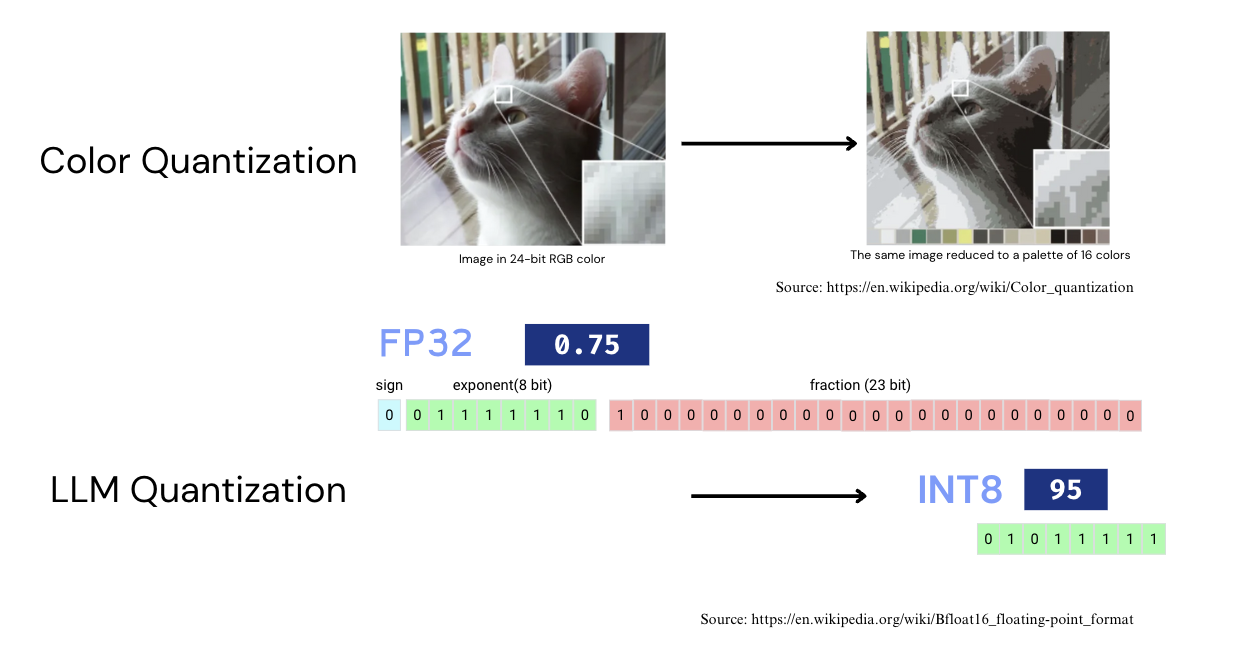
\includegraphics[width=\columnwidth]{img}
    \caption{Analogy Between Color Quantization and LLM Quantization}
    \label{fig:quantvisual}
\end{figure}

Quantization can be applied 1) during the training phase (\textit{QAT}) which is observed to be highly efficient; however, due to significant resource demands, oftentimes appears impractical \cite{chen2024EfficientQAT}, and 2) post-training (\textit{PTQ}), which is more resource efficient, but can lead to certain levels of performance degradation \cite{shen2024exploring}. To break it down further, quantization granularity levels can vary from per-tensor (one step for the entire matrix), to per-token  (scales per output token) and per-channel (channel step size)\cite{shen2024exploring}. Based on the module of the model that is being quantized, weight, activation and fixed-point quantization are distinguished \cite{bai2024beyond}.

Having established the theoretical foundation of quantization, we now provide an overview of key methods. \textit{GPTQ} (Generative Pre-trained Transformers Quantization) focuses solely on weights and aims to minimize quantization error through optimal weight rounding \cite{frantar2023GPTQ}. In contrast, \textit{AWQ} (Activation-aware Weight Quantization) assumes that weights carry varying levels of importance, therefore skipping crucial activation outliers while aggressively quantizing the rest helps mitigate accuracy loss \cite{lin2024AWQ}. \textit{GGUF}, in turn a successor of deprecated \textit{GGML}, includes  quantization-aware kernels optimizations and  provides backward-compatible file format among other improvements \cite{rajput2024benchmarking}. \textit{SmoothQuant} \cite{xiao2023SmoothQuant} enables quantization for both activations and weights by managing outlier values and QLoRA (4-bit quantized version of LoRA fine-tuning technique) \cite{dettmers2023qlora} reduces GPU requirements while still preserving performance.

Described techniques demonstrate superior advancements and efficiency, leading us to adopt GPTQ-, GGUF- and AWQ- quantized models in this study.

\section{Research Methodology}\label{method}

\subsection{Overview}

% - Describe and explain the research strategy (i.e. Surveys , Experiments , MSR , Case Study , Design Science , Action Research ). Motivate your choice of this method to address this problem.
% - Give a brief overview of the whole research method and the rest of the methodology section.
% - (For Experiments ) Describe independent/control/dependent variables, how the
% subjects were divided etc. Describe research questions as formal hypotheses


We perform \textbf{Experimentation}\cite{wohlin2012experimentation}, a research method commonly used
to explore empirical correlations between several factors, in our case,
quantized LLMs and their ability to create REST links. By the nature of
experiment, we have control over subjects, objects, and instrumentation in order
to manipulate experimental units and draw conclusions on dependent variable
output. Experiments are conducted to test the hypothesis and comparatively
access the impact of specific variables in a controlled setting, which is the
most suitable setup for answering our Research Questions.

Within a \textit{Controlled Experiment}, we aim to study the effect of
\textit{Independent Variables} (such as selected baseline LLM models and
quantization techniques) on \textit{Response Variables} (such as precision,
recall, F1-score, and others)\cite{wohlin2012experimentation}. In the design of
the experiment we defined a number of treatments, specific manipulations applied
to subjects\cite{wohlin2012experimentation}.  In this case, \textit{treatments}
involve a comparative evaluation of LLama, Mistral, and Mixtral in both their
non-quantized and quantized versions for REST alignment. These models were
previously used by Quinstedt and Lindgren, Ivarsson and Setterström and
al.\cite{quinstedt2024Optimizing},\cite{ivarsson2023automated} in their
respective studies. 

% FIXME: moved here from the introduction!
% .. with respect to their non-quantized
% \textit{base-model}\footnote{In this paper, a ``base'' model is one of the
% following: Mistral 7B Instruct-v0.2 (Mistral), Mixtral 8x7B Instruct-v0.1
% (Mixtral), and LLAMA 3 70B-Instruct (LLAMA 3).} counterparts.

% =*= HYPOTHESES =*=

% FIXME: something like this, but write it better
We consider \textbf{factor 1}: model (3 levels; LLama, Mistral, Mixtral);
\textbf{factor 2}: quantization technique (4 levels: None---``base'', GPTQ,
GGUF, AWQ). Hence, we generate 12 treatments labeled as $M_{i}$, with $1 \leq i
\leq 12$.

We define hypotheses for the experiment in the following way:
\begin{RQBox}
    \begin{itemize}
        \item $h_{0}$: There is no difference in performance between the treatments under test. $M_{1} = M_{2} = \dots = M_{12}$ (\textbf{RQ1}).
        \item $h_{a}$ There is a difference in performance between the treatments under test. $M_{1} \neq M_{2} \neq \dots \neq M_{12}$ (\textbf{RQ2}).
    \end{itemize}
    
    \textbf{Note: RQ3} is answered as a part of a descriptive trade-off
    analysis.
\end{RQBox}


% Added for A2 - Give a brief overview of the whole research method and the rest of the methodology section.
This section outlines the research type and structure, as well as evaluates the
appropriateness of scope in connection to identified \textbf{RQs}. Data
collection section defines procedures for sampling subjects of the study.
Further we explain and motivate the choice of methods and statistical tests we
use for data analysis and acknowledge identified threats to validity alongside
mitigation strategies.

\begin{center}
   \begin{center}
        \textbf{Experimental Design}
    \end{center}
    \begin{tcbraster}[raster columns=2, raster column skip=5pt, raster equal height=rows, raster row skip=5pt]
        \begin{roundedBox}
            \centering
            \textbf{Independent Variable (factors)}
            \begin{itemize}
                \item ``Base model''
                \item Level (treatment)
                    \begin{itemize}
                        \item GPTQ Quantization
                        \item GGUF Quantization
                        \item AWQ Quantization % Activation-aware Weight Quantization
                    \end{itemize}
            \end{itemize}
        \end{roundedBox}
        \begin{roundedBox}
            \centering
            \textbf{Objects (experimental units)}
            \begin{itemize}
                \item Hardware (Alvis)
                \item Alvis job-scripts
                \item REST-at tool
                % \item Hardware: local
            \end{itemize}
        \end{roundedBox}
        \begin{roundedBox}
            \centering
            \textbf{Dependent Variable (responses)}
            \begin{itemize}
                \item Accuracy
                \item Precision
                \item Recall
                \item $F1$-score
                \item Time-to-analyze
                \item GPU memory-usage (vRAM)
            \end{itemize}
        \end{roundedBox}
        \begin{roundedBox}
            \centering 
            \textbf{Control Variables (parameters)}
            \begin{itemize}
                \item Requirements file
                \item Test case file
                \item Ground truth file
                \item Prompt template
                \item Model hyper-parameters \\ (e.g. temperature)
                \item Python environment (version)
            \end{itemize}
        \end{roundedBox}
        \end{tcbraster}
        \begin{roundedBox}
            \centering
            \textbf{Output (artifacts)}
            \begin{itemize}
            \centering
                \item Structured trace links
            \end{itemize}
        \end{roundedBox}
\end{center}

\subsection{Data Collection}

% A) Describe and motivate data collection procedures, including how subjects are
% chosen (sampling), number of subjects, etc.
%   - Describe subjects (demographics, experience, etc.)
%
% B) Describe any instruments used in your study, e.g., interview guides,
% surveys, observation sheets, include these in your report (could be in appendix).
%
% C) Describe what types of data will be collected, is it qualitative,
% quantitative or both?
%
% D) What tooling, if any, will you use in the study (e.g., survey tool, MSR
% tool)
%
% E) Describe data collection procedures, sampling method(s), report the
% population and size of the sample.
% 
% F) If any instrument is used (e.g. document needed for the experiment,
% pre-questionnaire to check subjects background/experience, follow-up
% questionnaire), example questions/information from ALL of the needed instruments
% MUST be included.

For the scope of this study, we consider two datasets originating from Ericsson
AB and G\"oteborg Energi, respectively. These datasets serve as \textit{ground
truth} since they include the desired trace links established by the authors.
The requirement and software test pairs are sampled from each dataset to create
subsets ranging from 75 to 80 items using PRNG\footnote{Pseudo-random Number
Generator, cf. \url{https://epubs.siam.org/doi/abs/10.1137/0215025}}. This
sampling is performed to reduce overall computational costs. No human subjects
are involved in this phase beyond the authors of this paper, who oversee the
experiments in the event of technical difficulties. We gather the following
quantitative measures: (i) computed traces given (a) model and (b) dataset, and
(ii) benchmarks of job executions (i.e., running time, consumed resources).

Because of the stochastic nature of LLMs it is important that we perform
repeated tests on the same input for each of the models in order to be able to
include standard deviation measurements across the different metrics, this will
allow us to reason about the consistency of each model as well as increase the
validity of our measurements and subsequently our results.
% Question: If we repeat the test multiple times would the columns get multiplied by N in length or would this mean we have multiple different groups?

The software environment primarily employs the revised REST-at tool to collect
measurements resulting from individual job executions (i.e., the experiment).
These are conducted on the Alvis platform. For script execution, we use a
dedicated set of NVIDIA A100 Tensor Core
GPUs\footnote{\url{https://www.nvidia.com/en-us/data-center/a100/}} provided by the
platform. Consequently, all timing metrics are based on this hardware
configuration. After obtaining the measurements, we employ a post-processing
script that parses and consolidates outputs from all executions into a more
readable format.

\subsection{Data Analysis}

% - Describe and motivate the methods for analysing the data:
%  - Describe any quantitative data analysis that will be performed, if applicable.
%  – Describe the types of descriptive statistics you will use (e.g., data visualization, mean)
%  – This includes the types of statistical tests
%  and analysis you will apply and how you will interpret the results
% – Motivate the selection of statistical tests.

The collected data will be analyzed using the Wilcoxon signed-rank statistical
test: collected data is non-parametric---there are no assumptions about its
distribution---and paired---we will be comparing the same data points
(rows) between quantized and non-quantized model pairs
\cite{wohlin2012experimentation}. % TODO: mention that our nullH is two-sided

The data analysis will include confusion matrix performance indicators:
accuracy, precision, recall, F1-score, to be able to reason about the efficacy
of the model under test. The mean, median, and standard deviation will be
derived from the (repeated) tests for each model to give reliable measurements for
each of the different metrics. 

We perform pair-wise statistical analysis between the base model and their quantized counterparts, in order to show that any difference in performance is statistically significant, given that this is a gap in the current research. When examining the null hypotheses for each model pair, we can evaluate whether certain quantization techniques are more or less suitable depending on the measured performance. The alternative hypotheses can then be tested should the null hypotheses have been rejected, in order to confirm whether the quantized model version has significantly improved or declined performance. A descriptive analysis of the results will be used to analyze and discuss trade-offs of applied quantization. 
% Are there 2 or more groups however? What happens when we use levels of treatment, i.e., different quantization methods? -- seems like we would have > 2 groups

The data will be represented in tables comparing
the results from the different models. For this purpose, \textit{mean $\pm$ standard
deviation} will be displayed for each of the relevant metrics. Data will also be
represented using box-plots in order to visualize the distribution as well as
any outliers in each model's performance. 

% TODO: MENTION QUANTIZATION STRICTNESS -if we pair wise the base-model with the quantized models, assuming the quant models have more "aggressive" quantization applied, we could identify the "drop-off" point, i.e., when the quantized models start to significantly perform worse --- useful if they perform equally well up until some point 

\subsection{Threats to Validity}
% - Describe internal validity threats and mitigations.
% - Describe construct validity threats and mitigations.
% - Describe external validity threats and mitigations.
% - If applicable for your research method, describe further validity threats and mitigations under further categories.

% Ideas: 
Based on the guidelines proposed by Wohlin et al. \cite{wohlin2012experimentation} we identify the following threats to validity that might have influenced research findings: 
\subsection*{\textbf{1) Internal validity}}
    \textit{Response variability }- due to stochastic behavior of LLMs, the same prompt can result in different outputs when executed several times, this behavior can not be mitigated. Instead, we try to eliminate this risk by invoking prompts multiple times and defining consistent hyper-parameters.
    
    \textit{Selection of models} - in the process of selecting LLMs to be tested in this study, our aim was to ensure unbiased and fair judgment, although there is a possibility of influence of prevailing trends or widely accepted benchmarks.
    
    \textit{Quantized LLM quality} - in our study, we have utilized Quatized Models distributed via \textit{HuggingFace} platform, which might have limitations beyond our control. One of them is the parameter values and bias of the training source, which have a direct impact on the artifacts we obtained.
    % alternative -> explore using Alvis for quantizing models ourselves 

\subsection*{\textbf{2) External validity}}
    
    \textit{Domain-Specific Applicability} - the observed results might only be applicable within the explored domain due to the data specificity and scoped research questions.
    
    \textit{Results reproducibility on a local machine (this threat will be elaborated on in later stages of development, as it depends on the viability of a local environment setup for running the experiments. Otherwise, experiments will be conducted on the Alvis platform).}

\subsection*{\textbf{3) Construct validity}}
% \textit{    *concerns generalisation of the experiment result to concept or theory behind the experiment*
% }
\textit{Ground Truth Validity} - REST alignment mappings obtained from our Industry Partner have been fact-checked, verified, and as a result accounted for as ground truth; however, any potential bias, error, or human factor in its creation could have influenced the reliability of evaluation.

\section*{Acknowledgment}
We dedicate our gratitude to our supervisor Francisco Gomes and responsible for
the course in Research methods, Birgit Penzenstadler, for their valuable
insights. Moreover, we're thankful for the computing resource from Alvis offered
by the Chalmers Centre for Computational Science and Engineering 

\section*{Assignment 2: Work Delegation}

\begin{itemize}
    \item Erik: \ref{background}, \ref{relatedWork} A, \ref{method} C
    \item Mariia: Revised Quantization of LLMs \ref{relatedWork} B; Methodology Overview \ref{method} A, Threats to Validity \ref{method} D 
    \item Michal: Revised \ref{intro}, Abstract; Data Collection \ref{method}
\end{itemize}

\noindent
Additionally, all members of the group collectively participated in literature
review, proof-reading, refining research-questions, designing the experiment, and other tasks.

\subsection*{Changes since Assignment 1}

\noindent
Because the team members are continually getting more familiar with the research
and its objective, a lot of the text that was previously written is now,
unfortunately, obsolete (especially Introduction \ref{intro}). Highlighting
individual changes would be excessive and clutter the document. Instead we
highlight what has \underline{not} been changed:

\begin{itemize}
    \item Background \ref{background}
\end{itemize}

% =*= USE LATER SECTION =*=

% Subsection: Results(?)
% We reassess the existing tool and make minor modifications to ensure compliance
% with the latest framework requirements and improve code readiness. This updated
% version is referred to as ``revised'' \verb|REST-at|\footnote{This version of
% the tool can be accessed via \url{https://github.com/SEM25-BSc/REST-at}.
% A complete list of changes is noted below, cf. \ref{method}.}.
% Subsection: Discussion / Results
% Write about Scalability? How does it perform with 10, 20, 50, 100, entries?

% =*= USE LATER SECTION =*=

\bibliographystyle{IEEEtran}
\bibliography{lib}

\section*{Appendix}\label{appendix}

\end{document}